\section{Local Development}

\begin{frame}[plain,noframenumbering]
 \vfill
 \begin{center}
  \LARGE \color{solarizedAccent} Local Development
 \end{center}
 \vfill
\end{frame}

\begin{frame}
 \frametitle{Local Development}
 \framesubtitle{Forking}

 \begin{itemize}
  \item Push access to Geodynamics repos on GitHub restricted
  \item How to share code?
  \pause
  \item Create a \alert{fork} (personal GitHub copy of repo):
   \begin{tikzpicture}
    \node[anchor=south west, inner sep=0] at (0,0) {
     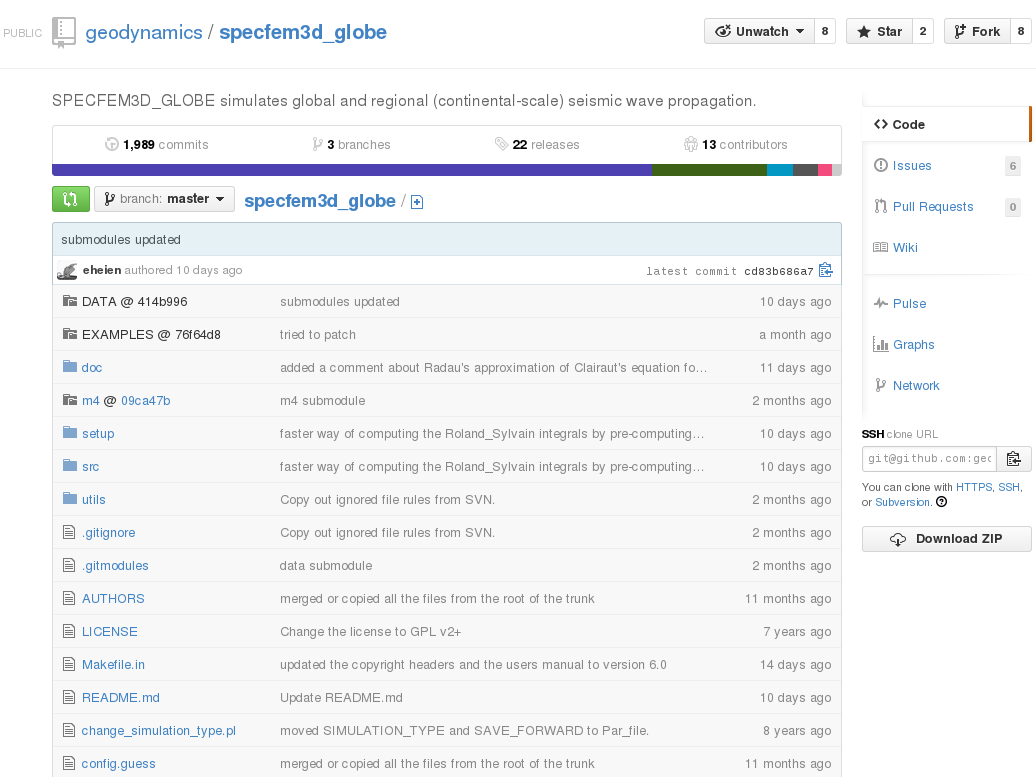
\includegraphics[width=\linewidth, height=\textheight, keepaspectratio,
                      trim={0 700px 0 0}, clip]{github}
    };
    \draw[solarizedAccent, thick, rounded corners]
     (9.1,0.3) rectangle (10.0,0.6);
   \end{tikzpicture}
 \end{itemize}
\end{frame}

\begin{frame}[fragile]
 \frametitle{Local Development}
 \framesubtitle{Forking}

 Set remotes for both repos (conventions):
 \begin{itemize}
  \item \texttt{origin} to your fork
  \item \texttt{upstream} to Geodynamics repo
 \end{itemize}

 \begin{exampleblock}{Setting Remotes}
  \begin{semiverbatim}
\comment{Clone \textit{your} fork}
\command{git clone -{}-recursive \\
   https://github.com/\alert{username}/specfem3d_globe.git}

\comment{Add remote for Geodynamics repo}
\command{git remote add upstream \\
   https://github.com/\alert{geodynamics}/specfem3d_globe.git}
\command{git fetch upstream}
\end{semiverbatim}
 \end{exampleblock}
\end{frame}

\begin{frame}[fragile]
 \frametitle{Local Development}
 \framesubtitle{Reviewing Changes}

 \begin{exampleblock}{Checking Status}
  \vspace{-1em}
  \begin{semiverbatim}
\command{git status}
On branch devel

Changes not staged for commit:
  (use "git add <file>..." to update what will be
   committed)
  (use "git checkout -{}- <file>..." to discard changes
   in working directory)
    \hiRed{modified:   DATA} (new commits)
    \hiRed{modified:   src/specfem3D/specfem3D.F90}

no changes added to commit (use "git add" and/or "git
commit -a")
\end{semiverbatim}
 \end{exampleblock}
\end{frame}

\begin{frame}[fragile]
 \frametitle{Local Development}
 \framesubtitle{Reviewing Changes}

 \begin{exampleblock}{Viewing Diffs}
  \vspace{-1em}
  \begin{semiverbatim}
\command{git diff \only<2->{master} \only<3>{-{}- src/}}\uncover<3>{
\textbf{\color{solarizedBase1}diff -{}-git a/src/specfem3D/specfem3D.F90 b/src/..
index 3ba52f2..2b619bf 100644
-{}-{}- a/src/specfem3D/specfem3D.F90
+++ b/src/specfem3D/specfem3D.F90}
\hiBlue{ @@ -466,6 +466,6 @@}
   ! sets up and precomputes simulation arrays
   call prepare_timerun()

\hiRed{-  ! steps through time iterations}
\hiGreen{+  ! Test change}
   if( UNDO_ATTENUATION ) then
     call iterate_time_undoatt()}
\end{semiverbatim}
 \end{exampleblock}
\end{frame}

\begin{frame}
 \frametitle{Local Development}
 \framesubtitle{Working with the Index}

 \begin{itemize}
  \item \alert{Index} or \alert{staging area} stores changes to be committed
  \item Option \texttt{-{}-cached} makes commands work in reference to index
  \begin{itemize}
   \item \texttt{git diff} compares index with working directory
   \item \texttt{git diff -{}-cached} compares HEAD with index
  \end{itemize}
 \end{itemize}
\end{frame}

\begin{frame}[fragile]
 \frametitle{Local Development}
 \framesubtitle{Working with the Index}

 \begin{exampleblock}{Adding New Files}
  \begin{semiverbatim}
\command{git add <new file>}
\end{semiverbatim}
 \end{exampleblock}

 \begin{exampleblock}<2->{Removing \textit{Existing} Files}
  \begin{semiverbatim}
\command{git rm <file>}
\end{semiverbatim}
 \end{exampleblock}

 \begin{exampleblock}<3>{Removing \textit{Newly Added} Files (i.e., from index)}
  \begin{semiverbatim}
\command{git rm -{}-cached <file>}
\end{semiverbatim}
 \end{exampleblock}
\end{frame}

\begin{frame}[fragile]
 \frametitle{Local Development}
 \framesubtitle{Working with the Index}

 \begin{exampleblock}{Adding Changes in Files}
  \begin{semiverbatim}
\comment{Add changes from file, patch-by-patch}
\command{git add -{}-patch} \comment{or -p}
\pause
\comment{Add entire change of file (not recommended)}
\command{git add <modified file>}
\pause
\comment{Add all changes of{\em tracked} files (not recommended)}
\command{git add -{}-all}
\end{semiverbatim}
 \end{exampleblock}
\end{frame}

\begin{frame}[fragile]
 \frametitle{Local Development}
 \framesubtitle{Working with the Index}

 \begin{exampleblock}{Undo Changes to Files}
  \begin{semiverbatim}
\comment{Remove changes to files}
\comment{(will match index)}
\command{git checkout -{}- <files>}
\pause
\comment{Remove changes from index}
\comment{(working directory unaltered)}
\command{git reset \uncover<3->{-{}- <files>}}
\pause\pause
\comment{Remove changes from files{\em and} index}
\command{git reset -{}-hard}
\end{semiverbatim}
 \end{exampleblock}
\end{frame}

\begin{frame}[fragile]
 \frametitle{Local Development}
 \framesubtitle{Committing}

 \begin{exampleblock}{Committing Changes in Index}
  \begin{semiverbatim}
\command{git commit}
\end{semiverbatim}
 \end{exampleblock}

 \begin{block}{Commit Messages}
\begin{verbatim}
Capitalized, short (50 chars or less) summary

More detailed explanatory text, if necessary.  Wrap
it to about 72 characters or so.  The blank line
separating the summary from the body is critical
(unless you omit the body entirely); tools like
rebase can get confused if you run the two together.
\end{verbatim}
 \end{block}
\end{frame}
